\section{USART}
    USART Addressraum:  \textbf{0x4001 3800 - 0x4001 3BFF}
    Für die USART muss, die Clock, die Bautrate, Parity, Wordlenght und die Interrupts eingestellt werden. 
    \subsection{Baudrate-Berechnung-Register-Setzen}
        Um die Baudrate einstellen zu können muss in das Register \textbf{USART\_BRR} die richtige Hexadezimal Zahl geschrieben werden.\\\\
        Berechnung: $\frac{Clock}{Baudrate}$, $\frac{8MHz}{38400}$ = 208,3$_{dezimal}$ bzw. D0$_{hex}$\\
        Zurückgerechnet $208*38400 = 7.98MHz. \frac{8MHz}{208} = $Baudrate von $38461$.\\\\
        Da der Systemclock gleich der HSI clock ist, kann dafür im Register \textbf{RCC\_CFGR3 bei der Addresse offset: 0x30} die USART1SW entweder 
        mit $01$ für Systemclock oder mit $11$ für HSI clock beschrieben werden. Zusätzlich muss im Register \textbf{USART\_BRR mit Address offset: 0x0C} D0 geschrieben
        Werden.
        
        \begin{figure}[!htb]
            \centering
            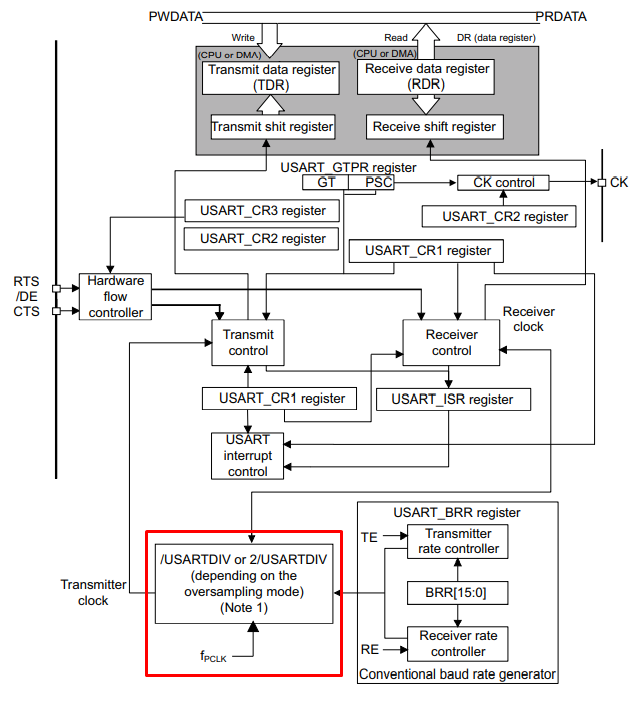
\includegraphics[scale=0.50]{USART-Aufbaug.png}
            \caption{USART-Aufbaug}
            \label{caption:USART-Aufbaug}
        \end{figure}
        \begin{figure}[!htb]
            \centering
            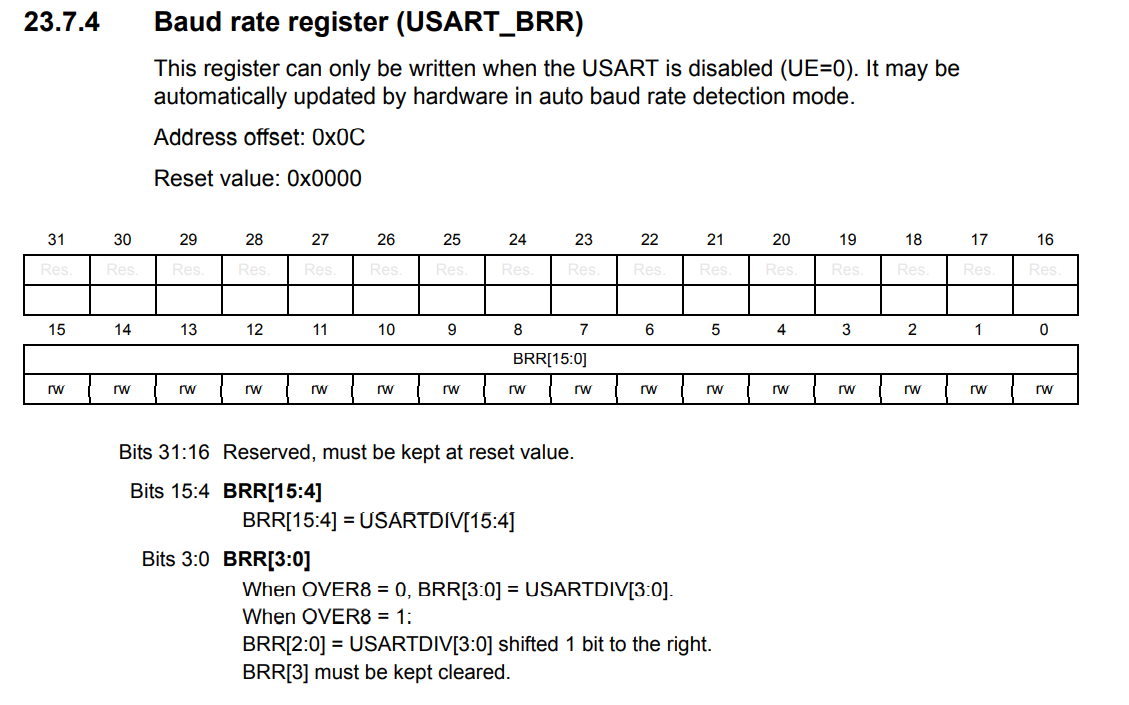
\includegraphics[scale=0.45]{USART-BRR.png}
            \caption{USART\_BRR}
            \label{caption:USART-BRR}
        \end{figure}
      
\newpage
    \subsection{Weitere USART einstellungen}
        Die Eistellungen der USART müssen getroffen werden, bevor sie aktiviert wird. Laut angabe wird noch eine ODD Parity verwendet diese kann in dem Register
        \textbf{USART\_CR1} auf Bit9: festgelegt werden. Weiterhin müssen dort unter Bit3 und Bit2, TX und RX aktivieren.

    \subsection{USART-Initiallisierung/Konfiguration|Code}
        \begin{lstlisting}[language=C, style=CStyle, caption=Init-UART, captionpos=b, label=Init-UART]
int init_UART()
{   
    uint32_t reg_content;
    uint32_t* rcc_cfr3 = RCC_CFGR3;
    uint32_t* usart1_brr = USART1_BRR;
    uint32_t* usart1_cr1 = USART1_CR1;

    //Use SYSCLK for USART and use Baudrate 38400
    reg_content = *rcc_cfr3;                
    reg_content |= 0x00000001;
    *rcc_cfr3 = reg_content; 
    
    reg_content = *usart1_brr;
    reg_content = 0x00000D00;
    *usart1_brr = reg_content;
    
    //Wordlenght, Parity control enable, Parity selection, interrupt enable, Transmission complete interrupt enable, RXNE interrupt enable
    reg_content = *usart1_cr1;
    reg_content |= 0x000006EC;
    *usart1_cr1 = reg_content;

    reg_content = *usart1_cr1;
    reg_content |= 0x00000001; //enable UART
    *usart1_cr1 = reg_content;
}
        \end{lstlisting}
        
    \subsection{USART-InterruptHandler}
    \begin{lstlisting}[language=C, style=CStyle, caption=Init-UART, captionpos=b, label=Init-UART]
void USART1_IRQHandler(void)
{   
    uint32_t* usart1_isr = USART1_ISR;
    uint32_t usart1_isr_rxne = USART1_ISR_RXNE;
    uint32_t usart1_isr_tc = USART1_ISR_TC;
    uint32_t* usart1_tc = USART1_ICR;
    uint32_t* usart1_tc_tcce = USART1_ICR_TCCF;
    uint32_t* usart1_tdr =  USART1_TDR;
    uint32_t* gpioa_odr = GPIOA_ODR;
    uint32_t reg_content;

    if ((*usart1_isr & usart1_isr_tc) == usart1_isr_tc)
    {
        if (send == sizeof(USART_write_data)) 
        {
            //set MAX to listen 
            reg_content = *gpioa_odr;
            reg_content |= 0x00000000;
            *gpioa_odr = reg_content;          
            send=0;
            *usart1_tc |= *usart1_tc_tcce; // Clear transfer complete flag *      
        }
        else
        {
            // clear transfer complete flag and fill TDR with a new char 
            *usart1_tdr = USART_write_data[send++];
        }
    }

    //when something comes at usart, begin to write the ADC Data 
    if ((*usart1_isr & usart1_isr_rxne) == usart1_isr_rxne)
    {
        USART_READ = *((char *)USART1_RDR);
        //Set PA7 and PA6 high for max to send data
        reg_content = *gpioa_odr;
        reg_content |= 0x000000C0;
        *gpioa_odr = reg_content;

        *usart1_tdr  = USART_write_data[0];
    }
}
    \end{lstlisting}
                

    
   